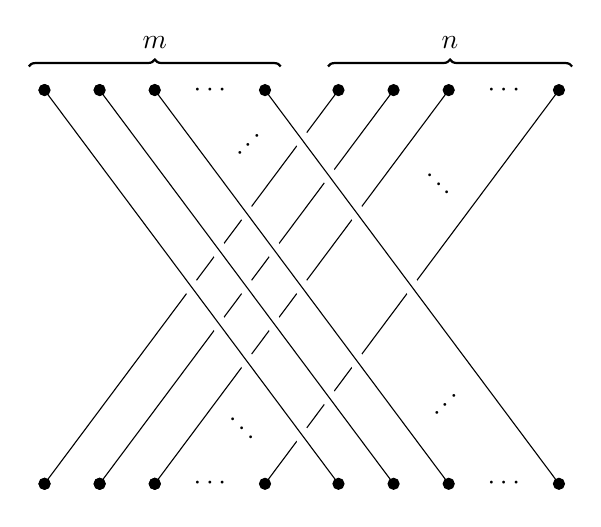
\begin{tikzpicture}
            \def\height{5}
            \def\ptsep{0.7}
            \def\sep{5.333}
            \tikzset{
                position label/.style={
                below = 3pt,
                text height = 2ex,
                text depth = 1ex
                }
            }
            
            

            
            \draw[thick, decoration={brace}, decorate] (-0.2,0.3) -- (3,0.3);
            \draw[thick, decoration={brace}, decorate] (3.6,0.3) -- (6.7,0.3);
            \node at (1.4, 0.6) {$m$};
            \node at (5.15, 0.6) {$n$};
            
            
            \foreach \x in {5.333, 6.333, 7.333}{
                \filldraw (\x*\ptsep, 0) circle (0.07cm); 
                \draw (\x*\ptsep,0) -- (\x*\ptsep - 5.333*\ptsep, -\height);
            }
            
            \node at (8.333*\ptsep, 0) {$\cdots$};
            \filldraw (9.333*\ptsep,0) circle (0.07cm); 
            \draw (9.333*\ptsep,0) -- (9.333*\ptsep - \sep*\ptsep, -\height);

            
            \foreach \x in {0, 1, 2}{
                \filldraw (\x*\ptsep, 0) circle (0.07cm); 
                \draw[line width = 2mm, white] (\x*\ptsep,0) -- (\x*\ptsep +\sep*\ptsep, -\height); 
                \draw (\x*\ptsep,0) -- (\x*\ptsep +\sep*\ptsep, -\height); 
            }
            
            \node at (3*\ptsep, 0) {$\cdots$};
            \draw (4*\ptsep,0) -- (4*\ptsep + \sep*\ptsep, -\height);
            \draw[line width = 2mm, white] (4*\ptsep,0) -- (4*\ptsep + \sep*\ptsep, -\height);
            \draw (4*\ptsep,0) -- (4*\ptsep + \sep*\ptsep, -\height);
            \filldraw (4*\ptsep,0) circle (0.07cm); 

            
            
            
            \foreach \x in {0, 1, 2}{
                \filldraw (\x*\ptsep, 0) circle (0.07cm); 
            }

            \foreach \x in {0, 1, 2}{
                \filldraw (\x*\ptsep, -\height) circle (0.07cm); 
            }
            
            \node at (3*\ptsep, -\height) {$\cdots$};
            \filldraw (4*\ptsep,-\height) circle (0.07cm); 

            \foreach \x in {0, 1, 2}{
                \filldraw (\x*\ptsep, -\height) circle (0.07cm); 
            }

            
            \foreach \x in {5.333, 6.333, 7.333}{
                \filldraw (\x*\ptsep, -\height) circle (0.07cm); 
            }
            
            \node at (8.333*\ptsep, -\height) {$\cdots$};
            \filldraw (9.333*\ptsep,-\height) circle (0.07cm); 


            \node at (5,-1.2) {\rotatebox{-45}{$\cdots$}};
            \node at (2.5,-4.3) {\rotatebox{-45}{$\cdots$}};
            \node at (2.6,-0.7) {\rotatebox{45}{$\cdots$}};
            \node at (5.1,-4) {\rotatebox{45}{$\cdots$}};
        \end{tikzpicture}